\documentclass[english, a4paper, 11pt]{article}
\usepackage[utf8]{inputenc}

%Margins 
\usepackage[a4paper, left=1.27cm,top=1.27cm,right =1.27cm, bottom = 1.4cm]{geometry}

%Load packages
%Algemene packages
\usepackage{babel}
\usepackage{slantsc}
\usepackage{array}
\renewcommand{\arraystretch}{2}
\usepackage{multicol}
\usepackage{multirow}
\usepackage{amsmath}
\usepackage{amsfonts}
\usepackage{booktabs}

%Opsommingen
\usepackage{enumerate}


%Afbeeldingen
\usepackage{graphicx}
\usepackage{wrapfig}

%Gekleurde tekstboxen 
\usepackage[most]{tcolorbox}

%Stop indent
\setlength{\parindent}{0pt}

%Font
\usepackage{cmbright}
\usepackage[OT1]{fontenc}

%Headers and footers
\usepackage{fancyhdr}

\pagestyle{fancy}
\fancyhf{}
\renewcommand{\headrulewidth}{0pt}
\renewcommand{\footrulewidth}{0pt}
\fancyhead[LE,RO]{}
\fancyhead[RE,LO]{}

%Logo in footer
\usepackage{lastpage}
\lfoot{}
\cfoot{\vspace{-5mm} \thepage}
\rfoot{}

%Voorbeeldtekst
\usepackage{lipsum}

%Meerdere kolommen
\usepackage{multicol}
\setlength{\columnsep}{1cm}

%Whitespace na section
\usepackage[compact]{titlesec}  
\titlespacing{\section}{0pt}{2pt}{0pt}

%Tekst kleur
\usepackage{xcolor}

%Nieuwe kleur
%\definecolor{ugent_blue}{rgb}{0.04706, 0.13725, 0.26667}
\definecolor{ugent_blue}{RGB}{30, 100, 200}

%Nummering sections
\renewcommand\thesection{\arabic{section}}
\renewcommand\thesubsection{\thesection.\arabic{subsection}}

%Lay-out hoofdingen
\titleformat*{\section}{\bfseries \normalfont}
\usepackage{sectsty}
\sectionfont{\color{ugent_blue}}
\titlespacing\section{0pt}{10pt plus 4pt minus 4pt}{0pt plus 2pt minus 2pt}

\raggedbottom


%other shit that may be useful
\usepackage{multicol,caption}
\usepackage{mathtools}
\raggedbottom
\newcommand{\HRule}{\hrule}
\abovedisplayskip0pt
\renewcommand{\arraystretch}{1.5}
\newcolumntype{M}[1]{>{\centering\arraybackslash}m{#1}}
\usepackage{lscape}
\newenvironment{Figure}
  {\par\medskip\noindent\minipage{\linewidth}}
  {\endminipage\par\medskip}
\usepackage{float}
\usepackage{hyperref}
\newcommand\myfigure[1]{%
\medskip\noindent\begin{minipage}{\columnwidth}
\centering%
#1%
%figure,caption, and label go here
\end{minipage}\medskip}
\usepackage{caption}
\usepackage{subcaption}
\usepackage{tabularx}
\usepackage{enumerate}
\usepackage{enumitem}

\raggedbottom
\raggedcolumns




\begin{document}

%Load heading of document
%ugent color
{\color{ugent_blue} \hrule\hrule\hrule}

\vspace*{-0.43mm}
\colorbox{ugent_blue}{\color{white} \bf Report Biomechanics}\\

\noindent\begin{minipage}{0.7\textwidth}% adapt widths of minipages to your needs
{\LARGE \bf \color{ugent_blue} Clinical Movement Analysis Lab Assignment 2022}\\[2mm]

%
{\large Vincent Belpaire}\\
{Supervisor: Prof. Malcolm Forward}\\


{\small University of Ghent}\\
{\small Faculty of Engineering and Architecture}\\
{\small Bachelor of Science: Biomedical Engineering}\\
\end{minipage}%
\hfill%
\begin{minipage}{0.3\textwidth}
\vspace{-2.2cm}
\begin{center}

\includegraphics[width=\linewidth]{ugent_logo}
\end{center}
\end{minipage}\\

\section{Introduction}

    This small report consists out of three parts - 3D marker trajectory, balance assessment and EMG - which 
    are not related to each other in the sense that one part does not depend on the resulst form another, i.e. each part is a stand alone.\\

    In each section data is used obtained form the \emph{Gait \& Movement Lab} at UZ Ghent. This data is stored in an excel file
    and is manipulated with python to create the necessary results. The used python code is based on the Jupyter Notebook file created by \emph{Juul Van Derbeken} 
    - for this a special thanks to him - and is further edited to match the style of this report.

    \begin{lstlisting}[language=Python, caption=imported python modules]
import numpy as np # data manipulation
import openpyxl # imorting data from excel
import matplotlib.pyplot as plt # data plotting
import scipy.signal as sg # signal analysis
    \end{lstlisting}

\section{3D marker trajectory}

    Three walk trials were recorded in the Lab.

    Using the \emph{openpyxl} module data can be easily imported in python for further manipulation. 
    Remark that in code block~\ref*{lst:3Dmtd} on the end of line 5 the first range starts from 14 instead of 5 this due 
    to NoneType elements contained in the range 5:14. Because it is just a small range compaired to the full dataset - consisting 
    from $\pm$500 rows - it is assumed that this will not heavily impact the results.

    \begin{lstlisting}[language=Python, caption=importing 3D marker trajectory data, label=lst:3Dmtd]
input_file = '.\Group 3B.xlsx'
workbook = openpyxl.load_workbook(input_file)
Sheets = workbook.sheetnames # Excel sheet Names

T1 = np.array([[el.value for el in rij] for rij in workbook[Sheets[0]].rows])[14:,2:].T #First Trial, None values for rows < 14
T2 = np.array([[el.value for el in rij] for rij in workbook[Sheets[1]].rows])[5:,2:].T #Second Trial
T3 = np.array([[el.value for el in rij] for rij in workbook[Sheets[2]].rows])[5:,2:].T #Third Trial
T = [T1, T2, T3]
    \end{lstlisting}

    \subsection{Walking speed}

        For each trial the forward propagation direction is plotted in figure \ref*{fig:trajectory}.
        Note that on each plot multiple trajectory lines occur. Each line corresponds to a marker placed
        on the subject who executed these trials. The global (average) walking speed is then calculated as the mean
        of the different marker speeds. The results are placed in table \ref*{tab:walking_speed}.

        \begin{lstlisting}[language=Python, caption=walking speed calculation and trajectory plotting]
fig, ax = plt.subplots(1,3, figsize = (18,6),sharey=True)
ax[0].set_ylabel('distance in mm', fontsize=15)

for i, t in enumerate(T):
    AS = [] # average speeds
    for y in t[1::3]:
        v = np.diff(y) # instantanious speeds
        ASL = np.mean(v) # averaged speed
        AS.append(ASL)
        ax[i].plot(y), ax[i].set_title(f'trial {i+1}', fontsize=15)
    
    AS = np.array(AS) 
    speed = np.mean(AS) # Averaged speed for all markers
    std = np.std(AS)
    print(f'Average speed for Trial {i} = ',speed, ' and std = ', std)
plt.show()
        \end{lstlisting}

        \begin{figure}[!h]
            \centering
            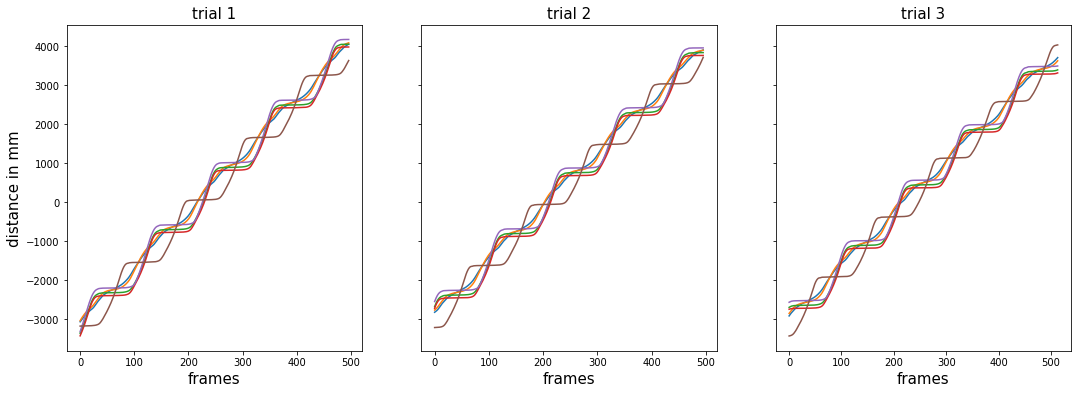
\includegraphics[scale=0.45]{direction_of_movement.png}
            \caption{forward propagation direction}
            \label{fig:trajectory}
        \end{figure}

        \begin{table}[!h]
            \centering
            \begin{tabular}{c|c|c}
                trial & walking speed [mm/frame] & std [mm/frame]\\ \hline
                1 & 14.58 & 0.48\\
                2 & 13.42 & 0.32\\
                3 & 12.61 & 0.97
            \end{tabular}
            \caption{Walking speed for different trials}
            \label{tab:walking_speed}
        \end{table}

    \subsection{Stride length}

        The stride length is calculated as the difference in foward propagation direction values corresponding to the local minima of the
        ankle marker height. To approximate these local minima a treshold is used as displayed in figure \ref*{fig:height}. The numerical results
        are listed in table \ref*{tab:stride_length}.

        \begin{lstlisting}[language=Python, caption=plotting marker height with treshold and calculating stride length]
fig, ax = plt.subplots(1,3, figsize = (18,6),sharey=True)
ax[0].set_ylabel('Height in mm', fontsize=15)
AHS = [] # average stride length for each trial. 
for i, t in enumerate(T):
    TAZ = t[8] # Trial Ankle Z-coordinate
    TAY = t[7] # Trial Ankle Y-coordinate (forward movement direction)
    Tp = np.percentile(TAZ, 30) # Treshold at 30%
    TP = np.ones(np.shape(TAZ))*Tp # treshold for graph
    P = np.where(TAZ < Tp, 1, 0) # ones where Trial is under treshold value
    HS = np.where(np.diff(P) == 1) # locations where values dip under treshold values. 
    Y = TAY[HS]
            
    ax[i].plot(TAZ), ax[i].plot(TP)
    ax[i].legend(['Data', 'Treshold'], loc="upper right", fontsize=15)
    ax[i].set_title(f"Trial {i+1}: Ankle", fontsize=15)
    print(np.diff(Y))
    print(f'Trial {i+1}: Average stride length is: ', np.mean(np.diff(Y)), " and std = ", np.std(np.diff(Y)))
plt.show()
        \end{lstlisting}

        \begin{figure}[!h]
            \centering
            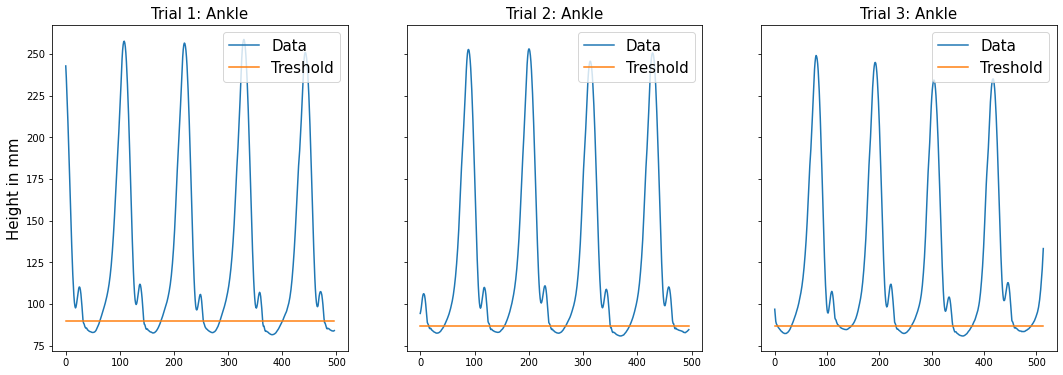
\includegraphics[scale=0.45]{z-coordinate.png}
            \caption{Ankle marker height}
            \label{fig:height}
        \end{figure}

        \begin{table}[!h]
            \centering
            \begin{tabular}{c|c|c}
                trial & walking speed [mm] & std [mm]\\ \hline
                1 & 1597.86 & 20.73\\
                2 & 1554.80 & 19.87\\
                3 & 1503.08 & 55.59
            \end{tabular}
            \caption{Stride length}
            \label{tab:stride_length}
        \end{table} 

The stride length is in the first place related to the person's height, since taller humans can take larger steps.
\section{Balance assessment}

    \begin{lstlisting}[language=Python, caption=importing balance assessment data, label=code:BA_input]
input_file = '.\Grp 3B Wk 2.xlsx'
workbook = openpyxl.load_workbook(input_file)
sheets = G2A_2.sheetnames #Sheet Names

EO = np.array([[el.value for el in rij] for rij in workbook[sheets[1]].rows])[6:15006,2:].T #First Trial #15006
EC = np.array([[el.value for el in rij] for rij in workbook[sheets[2]].rows])[6:12976,2:].T #Second Trial #12976

EOFX, EOFY, EOFZ = EO[0], EO[1], EO[2] # Eyes Open Force Vectors of x,y,z coordinates
ECFX, ECFY, ECFZ = EC[0], EC[1], EC[2] # Eyes Closed Force Vectors of x,y,z coordinates
    \end{lstlisting}

    First it is recommended to plot the overal xy-plane with the center of pressures (CoP) on it. This is displayed in figure \ref*{fig:CoP}.
    This gives a first impression between the two cases.

    \begin{lstlisting}[language=Python, caption=plotting CoP]
fig, (ax0, ax1) = plt.subplots(1,2, figsize = (18,6), sharey=True)
ax0.scatter(EOFX, EOFY, s=1), ax0.set_title('eyes open (EO)', fontsize=15), ax0.set_xlabel('x-coordinate in mm', fontsize=15), ax0.set_ylabel('y-coordinate in mm', fontsize=15)
ax1.scatter(ECFX, ECFY, s=1), ax1.set_title('eyes closed (EC)', fontsize=15), ax1.set_xlabel('x-coordinate in mm', fontsize=15)
plt.show()
    \end{lstlisting}

    \begin{figure}[!h]
        \centering
        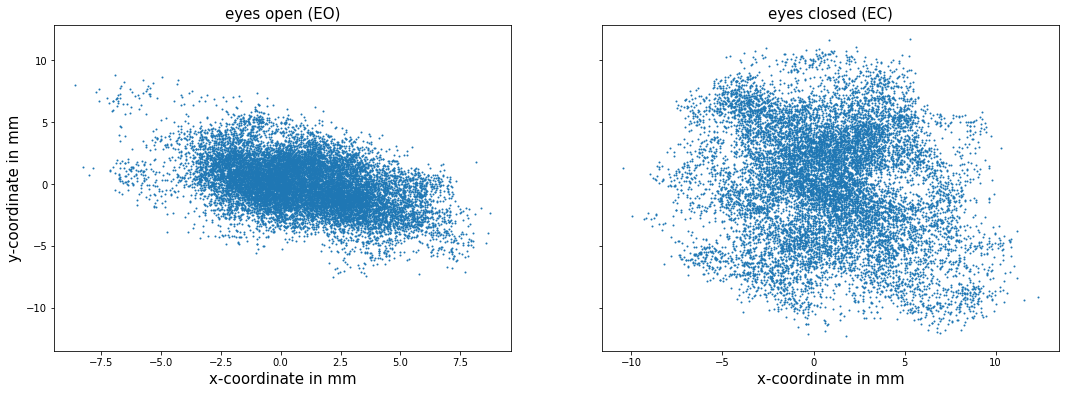
\includegraphics[scale=0.45]{CoP.png}
        \caption{Center of pressure}
        \label{fig:CoP}
    \end{figure}

    Different parameters such as path length, swept area and mean radius suffice to make a distinguishment between EO and EC.
    Before one of these parameters can be calculated one must calculate the Arithmetic Mean Point (AMP) and shift the axis
    to this point in space. The results of the three mentioned parameters are listed in table \ref*{tab:params}.

    \begin{table}[!h]
        \centering
        \begin{tabular}{c|c|c|c}
            trial & path length [mm] & swept area [mm$^2$] & mean radius [mm]\\ \hline
            EO & 15508.36 & 13936.26 & 2.879\\
            EC & 13462.69 & 22494.91 & 5.248
        \end{tabular}
        \caption{Calculated parameters}
        \label{tab:params}
    \end{table}

    \begin{lstlisting}[language=Python, caption=calculating the parameters]
def AMP(x): # calculating AMP
    return np.mean(x)

EOFXs, EOFYs = EOFX - AMP(EOFX), EOFY - AMP(EOFY) # shifting to AMP
ECFXs, ECFYs = ECFX - AMP(ECFX), ECFY - AMP(ECFY) # shifting to AMP

def Mean_radius(x, y):
    r = (x**2 + y**2)**(1/2) # radius
    return np.mean(r), np.std(r)

def Path_length(x, y):
    L = (np.diff(x)**2+np.diff(y)**2)**(1/2) # length
    return np.sum(L)

def Swept_area(x, y):
    r = (x**2 + y**2)**(1/2) # radius
    L = (np.diff(x)**2+np.diff(y)**2)**(1/2) # length
    a, b, c = L, r[:-1], r[1:]
    S = 1/2*(a+b+c)
    A = (S*(S-a)*(S-b)*(S-c))**(1/2)
    return np.sum(A)
    \end{lstlisting}

In table \ref*{tab:params} one migth expect every parameter to be larger in the EC scenario but instead the path length
reaches the highest value. Probably this is due to the difference in data points - more data points imply a longer path that can be passed.
Looking to code block \ref*{code:BA_input} one can observe on line 5 and 6 a great difference in data points between EO and EC (15006 $>$ 12976).\\

Some practical notes have to be taken into account for these measurements. The force plate
exists out of a collection of sensors. There can be small errors on the linearity of these 
sensors, i.e. the amount of displacement measured is not fully proportional with the measured voltage, which
leads to small errors in the data. It is crucial to minimalize these erros for accurate measurements.
Moreover do the number of sensors also influence the accuracy by which there can be measured.

Besides these practical limitations, there is also a choice to be made by the executor of the measurement, namely which sampling rate to use.
There are two factors to take into account: what is the maximal sampling rate the force plate can physically handle and by which frequencies does the subject on the force plate move.
Since the subject on the force plate is human it wise to start by looking at the human movement frecueny and to aim the sampling rate 
somewhere in between this human movement frecueny and the maximal sampling rate. A higher sampling rate would cause more noise
in the data, hence aiming to lower sampling rates that still would capture all the human movement is the goal.

\section{EMG}

    \begin{lstlisting}[language=Python, caption=input EMG data]
G2A_3_input = '.\G3B_EMG Lab3.xlsx'
G2A_3 = openpyxl.load_workbook(G2A_3_input)
SN3 = G2A_3.sheetnames #Sheet Names

EN = np.array([[el.value for el in rij] for rij in G2A_3[SN3[0]].rows])[11:10951,2:].T #EMG Normal walking #10951
ET = np.array([[el.value for el in rij] for rij in G2A_3[SN3[1]].rows])[11:11891,2:].T #EMG Toe walking #11891
    
    \end{lstlisting}


    \begin{lstlisting}[language=Python, caption=raw EMG plotting]
ENG = EN[0]- EN[1] #EMG Normal-walking Gastrocnemius
ENT = EN[2] - EN[3] #EMG Normal-walking Tibialis-anterior
ETG = ET[0]- ET[1] #EMG Toe-walking Gastrocnemius
ETT = ET[2] - ET[3] #EMG Toe-walking Tibialis-anterior        

fig, ((ax0, ax1), (ax2,ax3)) = plt.subplots(2,2, figsize = (14,8),sharey=True)
ax0.plot(ENG), ax0.set_title('Gastrocnemius Normal', fontsize=15), ax0.set_xlim(0,10000), ax0.set_ylabel('Voltage [V]', fontsize=15)
ax1.plot(ETG), ax1.set_title('Gastrocnemius Toe', fontsize=15), ax1.set_xlim(0,10000)
ax2.plot(ENT), ax2.set_title('Tibialis Ant Normal', fontsize=15), ax2.set_xlim(0,10000), ax2.set_ylabel('Voltage [V]', fontsize=15)
ax3.plot(ETT), ax3.set_title('Tibialis Ant Toe', fontsize=15), ax3.set_xlim(0,10000)
    \end{lstlisting}

    \begin{figure}[!h]
        \centering
        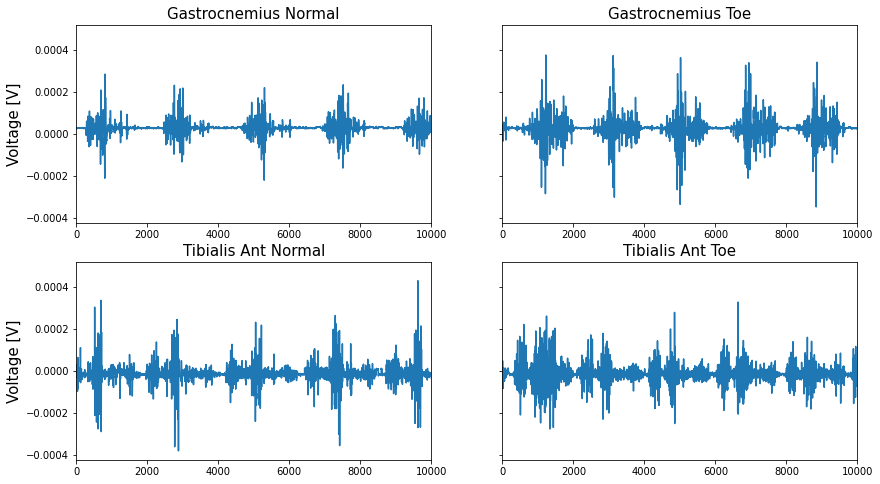
\includegraphics[scale=0.5]{EMG_raw.png}
        \caption{raw EMG signals}
        \label{fig:EMG_raw}
    \end{figure}

Looking at figure \ref*{fig:EMG_raw}, capturing the raw EMG data, the following obeservatoins can be made:
the separation between voltage bursts is shorter and the amplitudes reach higher values in the toe walking case
in comparison with the normal walking case.

    \begin{lstlisting}[language=Python, caption=rectified EMG calculation and plotting]
ENG = ENG - np.mean(ENG)
ENT = ENT - np.mean(ENT)
ETG = ETG - np.mean(ETG)
ETT = ETT - np.mean(ETT)
ENG, ENT, ETG, ETT = abs(ENG), abs(ENT), abs(ETG), abs(ETT)

fig, ((ax0, ax1), (ax2,ax3)) = plt.subplots(2,2, figsize = (14,8),sharey=True)
ax0.plot(ENG), ax0.set_title('Gastrocnemius Normal', fontsize=15), ax0.set_xlim(0,10000), ax0.set_ylabel('Voltage [V]', fontsize=15)
ax1.plot(ETG), ax1.set_title('Gastrocnemius Toe', fontsize=15), ax1.set_xlim(0,10000)
ax2.plot(ENT), ax2.set_title('Tibialis Ant Normal', fontsize=15), ax2.set_xlim(0,10000), ax2.set_ylabel('Voltage [V]', fontsize=15)
ax3.plot(ETT), ax3.set_title('Tibialis Ant Toe', fontsize=15), ax3.set_xlim(0,10000)
plt.show()
    \end{lstlisting}

    \begin{figure}[!h]
        \centering
        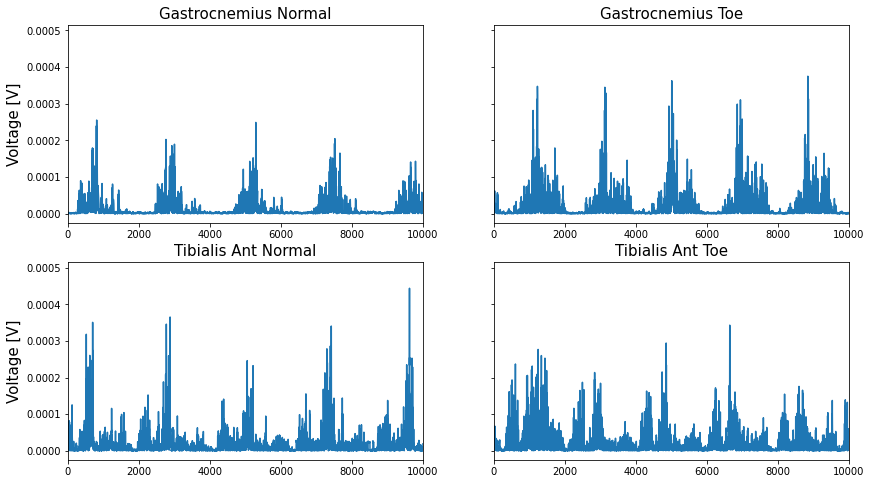
\includegraphics[scale=0.5]{EMG_rectified.png}
        \caption{rectified EMG signals}
        \label{fig:EMG_rect}
    \end{figure}

Starting from the rectified EMG signals, i.e. the absolute value taken from the original signals, one could produce smooth rectified EMG by filtering out the high frequencies in the signal. 
This can be realized with a low-band pass filter.\\
At last if one would want to deduce the resting EMG level, i.e. the measured voltage without the muscle actually being contracted, one should establish a threshold of EMG on/off levels.
This can be derived from the smoothed out rectified EMG signal. The voltages below this threshold can be considered as the resting EMG level.

\end{document}
